\documentclass[a4paper]{article}
\usepackage {graphicx}
\usepackage {hyperref}
\usepackage [inner=0.5cm,outer=0.5cm]{geometry}
\usepackage {mathtools}
\usepackage {subfig}

\topmargin=-3.5cm
\begin {document}

\title {BSP Parallel Computation of Convex Hull}
\author {Dmitri Kovalenko}

\maketitle
\section {Problem formulation}
    We are given set $S$ of 2D points. Goal is to construct set $CH(S)$, which is convex hull for $S$.\\
    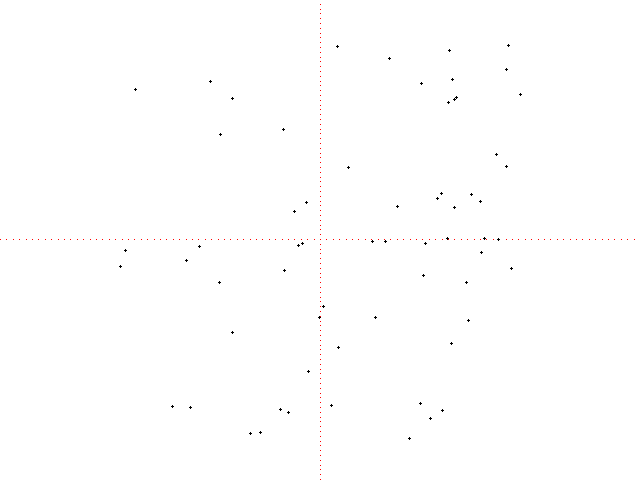
\includegraphics [width=0.45\textwidth] {plain_points.png}
    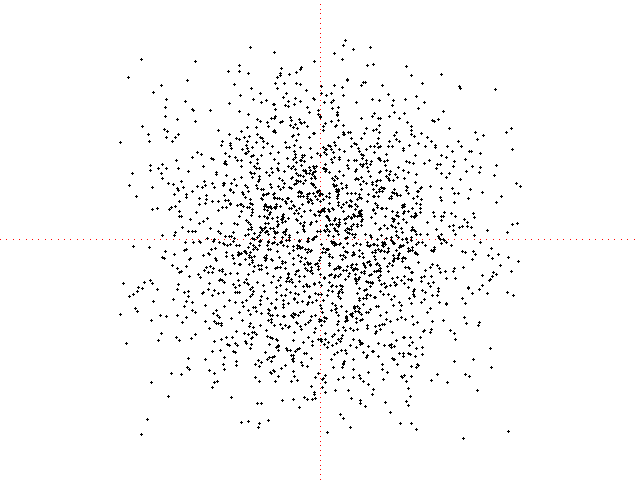
\includegraphics [width=0.45\textwidth] {plain_points_b.png}\\
    Expected results are listed below.\\
    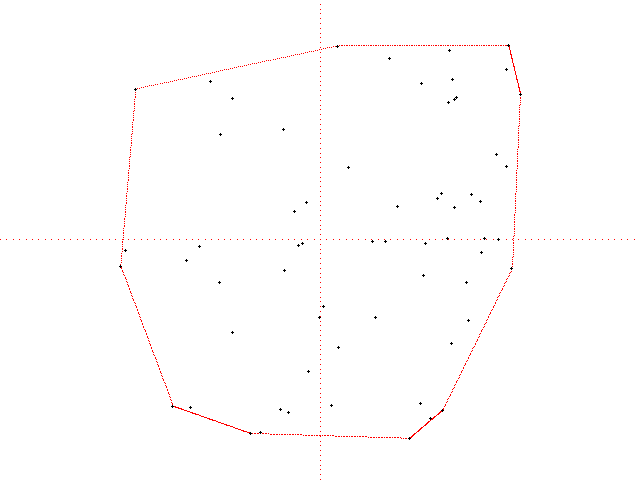
\includegraphics [width=0.45\textwidth] {final_hull.png}
    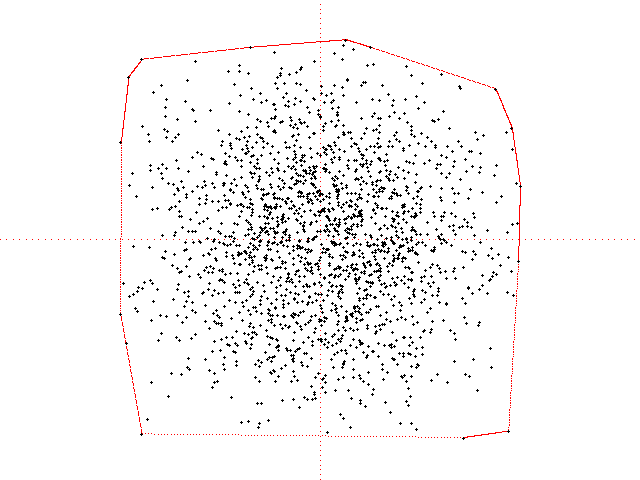
\includegraphics [width=0.45\textwidth] {final_hull_b.png}\\

\section {Algorithm description}
    Algorithm is heavely based on the solution sketch provided on the CS341 slides.\\
    Let $S$ - input set; $|S| = n$, $p$ - amount of processors available on parallel machine.\\
    We would name processor with index 0 the lead processor.\\
    \textbf {Algoritm steps}
    \begin {enumerate}
        \item Lead processor reads $n$ points from standard input
        \item All processors fetch $\frac n p$ points. These points are named \textit{local pointset}
        \item Compute hull of local pointset;
        \item Sample with regular interval $p$ points on the \textit{local hull}.
        \item Accumulate all samples on the lead processor. This would result \textit{samples set} of size $p^2$. \textit{Samples set} is an $\frac 1 p$-approximation of $S$.
        \item Lead processor calculates $\frac 1 p$-net of \textit{samples set}. This net would be called \textit{splitters} and appers to be $\frac 2 p$-net of whole pointset $S$.
        \item Lead processor broadcasts \textit{splitters} to all
        \item As any e-net, \textit{splitters} take the convex position, and might be seen as convex polygon. Under assumption that polygon is opaque, we may call a $\text{bucket}_i$ such subset of $S$, so allpoints of $\text{bucket}_i$ are visible from point $s_i$, $s_i \in \text{splitters}$. Each bucket defined by 2 halfspaces. Bind 2 buckets to each processor
        \item Each processors scans its \textit{local hull} and sends every point to corresponding bucket
        \item Compute local hulls of buckets sequentially
        \item Accumulate hulls on the lead processor, reject interior edges
        \item Output resulting hull to the standard output
    \end {enumerate}

\section {Code description}
     Implementation of the algorithm stored in the "parallel" repo under "\verb|/convex_hull/src|" folder.
     \begin {itemize}
         \item For the role of sequential convex hull algorithm graham scan was used
         \item Main steps of processing separated as methods of class \verb|parall_2d_hull|. So, Step 2 implemented in \verb|distribute_input|. 
         \item Step 3,4 implemented in \verb|compute_local_samples|
         \item Step 5 implemented in \verb|collect_all_samples|
         \item Step 6,7 implemented in \verb|compute_enet|
         \item Step 8,9 implemented in \verb|distribute_over_buckets|
         \item Step 10,11  implemented in \verb|accumulate_buckets|. Current version of this phase is simplified and lacks interior-edge rejection algorithm. Instead, one hull of all buckets is done on the lead processor
     \end {itemize}
\section {Computation illustration}
    Section is dedicated to illustrate processing steps from above.\\
    \begin{figure}
        \centering
        \subfloat[input]{\label{ref_label1}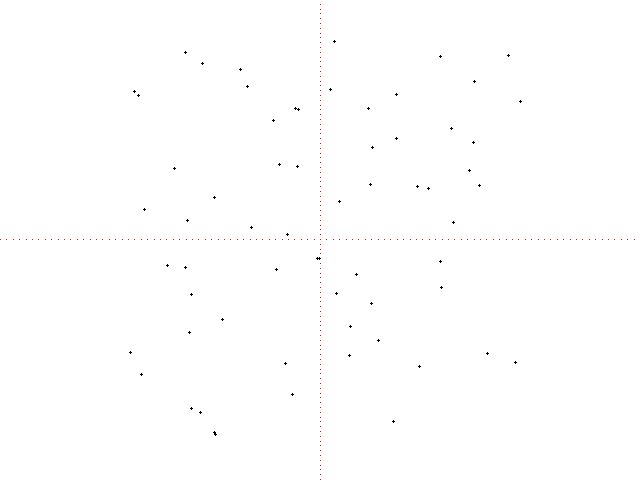
\includegraphics[width=0.45\textwidth]{illustration/plain_points.png}}
        \subfloat[$\frac 1 p$-approximation of $CH(S)$, \textit{samples set}]{\label{ref_label2}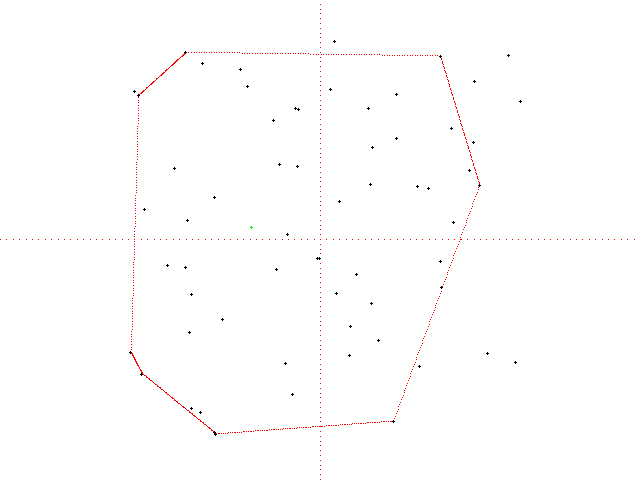
\includegraphics[width=0.45\textwidth]{illustration/hull_from_samples.png}}
    \end{figure}
    \begin{figure}
        \centering
        \subfloat[Process of enet computation.]{\label{ref_label1}
            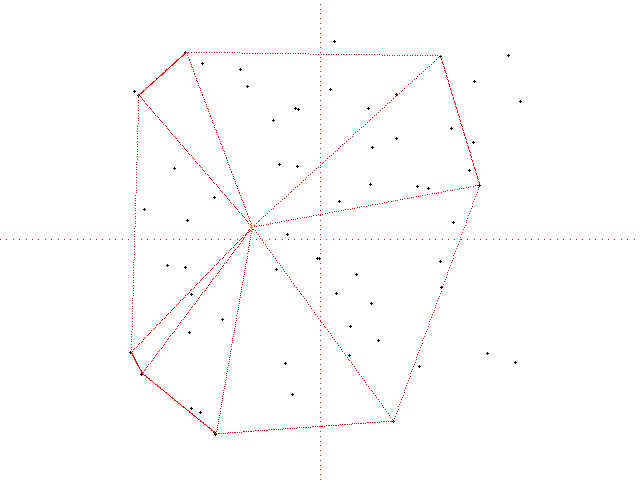
\includegraphics[width=0.45\textwidth]{illustration/tri.png}}
        \subfloat[$\frac 2 p$-net of $CH(S)$. Splitters]{\label{ref_label2}
            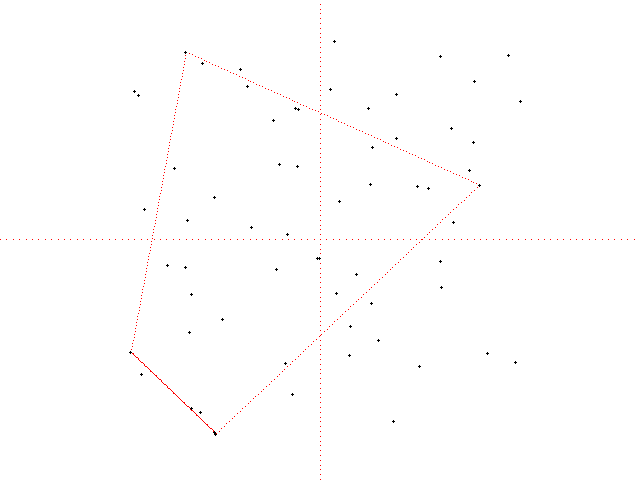
\includegraphics[width=0.45\textwidth]{illustration/splitters.png}}
    \end{figure}
    \begin{figure}
        \centering
        \subfloat[Example of filling a bucket]{\label{ref_label1}
            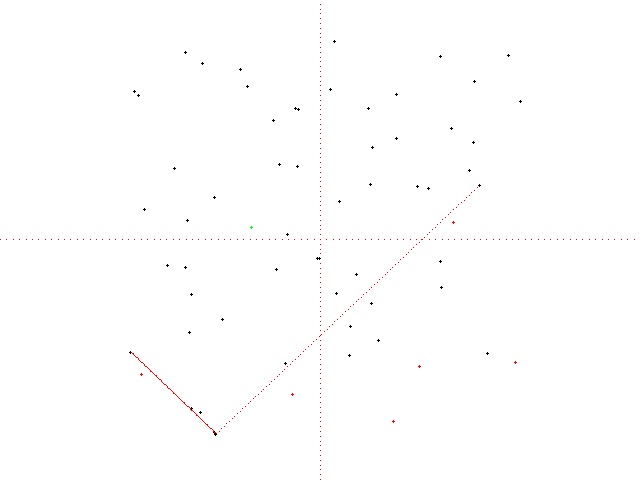
\includegraphics[width=0.45\textwidth]{illustration/bucket_0.png}}
        \subfloat[Result]{\label{ref_label2}
            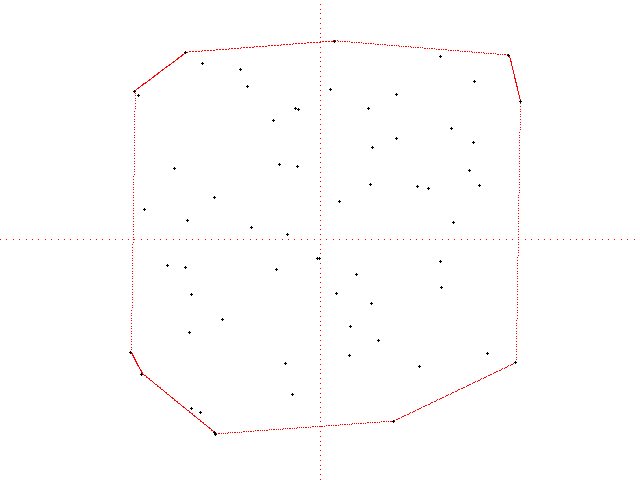
\includegraphics[width=0.45\textwidth]{illustration/final_hull.png}}
    \end{figure}
\section {References}
    \begin {enumerate}
        \item A. Tiskin "Advanced Topics in Algorithms" \url{http://www2.warwick.ac.uk/fac/sci/dcs/teaching/material/cs341/ata_handout1.pdf}
        \item A. Tiskin "Parallel Convex Hull Computation by Generalised Regular Sampling" 2002
        \item M. Diallo et al. "Scalable 2d Convex Hull and Triangulation Algorithms for Coarse Grained Multicomputers"
        \item M. Goodrich et al. "Randomized Fully-Scalable BSP Techniques for Multi-Searching and Convex Hull Construction" 1997
        \item J.Zhou et al. "A 2-D Parallel Convex Hull Algorithm with Optimal Communication Phases"
        \item R. Sujithan "BSP Parallel Sorting by Regular Sampling - Algorithm and Implementation"
    \end {enumerate}

\end {document}
